\section{Giới thiệu}

\subsection{Tóm tắt đề tài}
Đề tài tập trung nghiên cứu bài toán \textbf{Person Re-identification (ReID)} trong lĩnh vực Thị giác máy tính, với mục tiêu nhận dạng lại một người qua nhiều camera khác nhau. Trên cơ sở khảo sát các nghiên cứu liên quan, đề tài hướng đến việc đề xuất một mô hình dựa trên học sâu, thực nghiệm trên tập dữ liệu chuẩn và đánh giá hiệu quả bằng các độ đo phổ biến. Bên cạnh đó, đề tài cũng xem xét một số hướng cải tiến nhằm nâng cao hiệu quả nhận dạng.

\subsection{Bối cảnh bài toán}
Cùng với sự phát triển của các hệ thống giám sát thông minh, bài toán nhận dạng con người qua nhiều camera ngày càng nhận được nhiều sự quan tâm trong lĩnh vực Thị giác máy tính. Trong các môi trường như sân bay, nhà ga, trung tâm thương mại hay khu vực công cộng, một người có thể xuất hiện ở nhiều camera khác nhau với các điều kiện quan sát không đồng nhất. Do đó, việc xác định các hình ảnh thu được từ nhiều camera có thuộc cùng một người hay không là một bài toán có ý nghĩa thực tiễn cao.

\begin{figure}[!htbp]
    \centering
    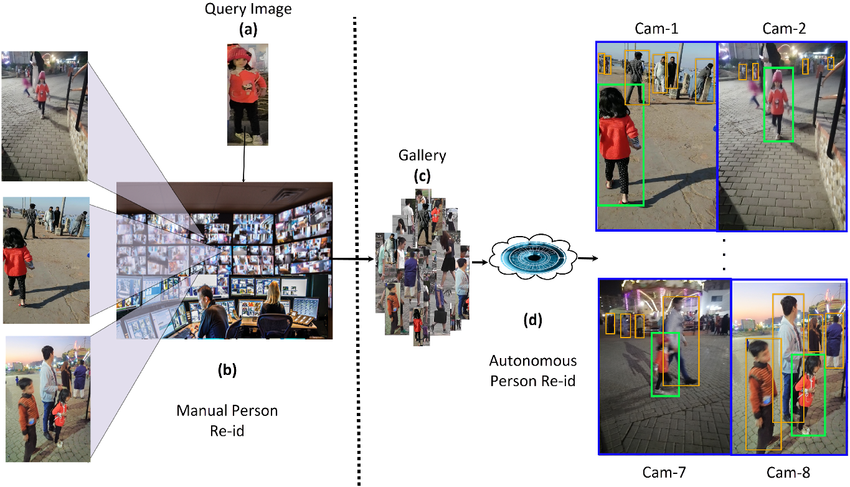
\includegraphics[width=0.7\textwidth]{img/smart-person-re-identification.png}
    \caption{Minh họa bài toán Person Re-identification trong hệ thống giám sát nhiều camera.}
    \label{fig:reid_example}
\end{figure}
Bài toán này được gọi là \textbf{Person Re-identification (ReID)}. Mục tiêu của Person ReID là tìm kiếm hoặc xác định lại một người trong tập ảnh hoặc video được thu thập từ nhiều camera khác nhau. Đây là một hướng nghiên cứu quan trọng, có nhiều ứng dụng trong giám sát an ninh, phân tích hành vi và quản lý di chuyển trong không gian công cộng.

Tuy nhiên, Person Re-identification là một bài toán khó do sự thay đổi lớn về góc nhìn, ánh sáng, tư thế, độ phân giải ảnh và hiện tượng che khuất giữa các camera. Bên cạnh đó, sự tương đồng về trang phục hoặc ngoại hình giữa nhiều người khác nhau cũng làm gia tăng khả năng nhầm lẫn.

\subsection{Vấn đề nghiên cứu}
Trong những năm gần đây, các phương pháp học sâu đã cho thấy hiệu quả nổi bật trong bài toán Person Re-identification nhờ khả năng học đặc trưng trực tiếp từ dữ liệu. Tuy vậy, hiệu quả của mô hình vẫn chịu ảnh hưởng bởi sự đa dạng của dữ liệu, khả năng biểu diễn đặc trưng và cách đo lường độ tương đồng giữa các đối tượng.


\begin{figure}[!htbp]
    \centering
    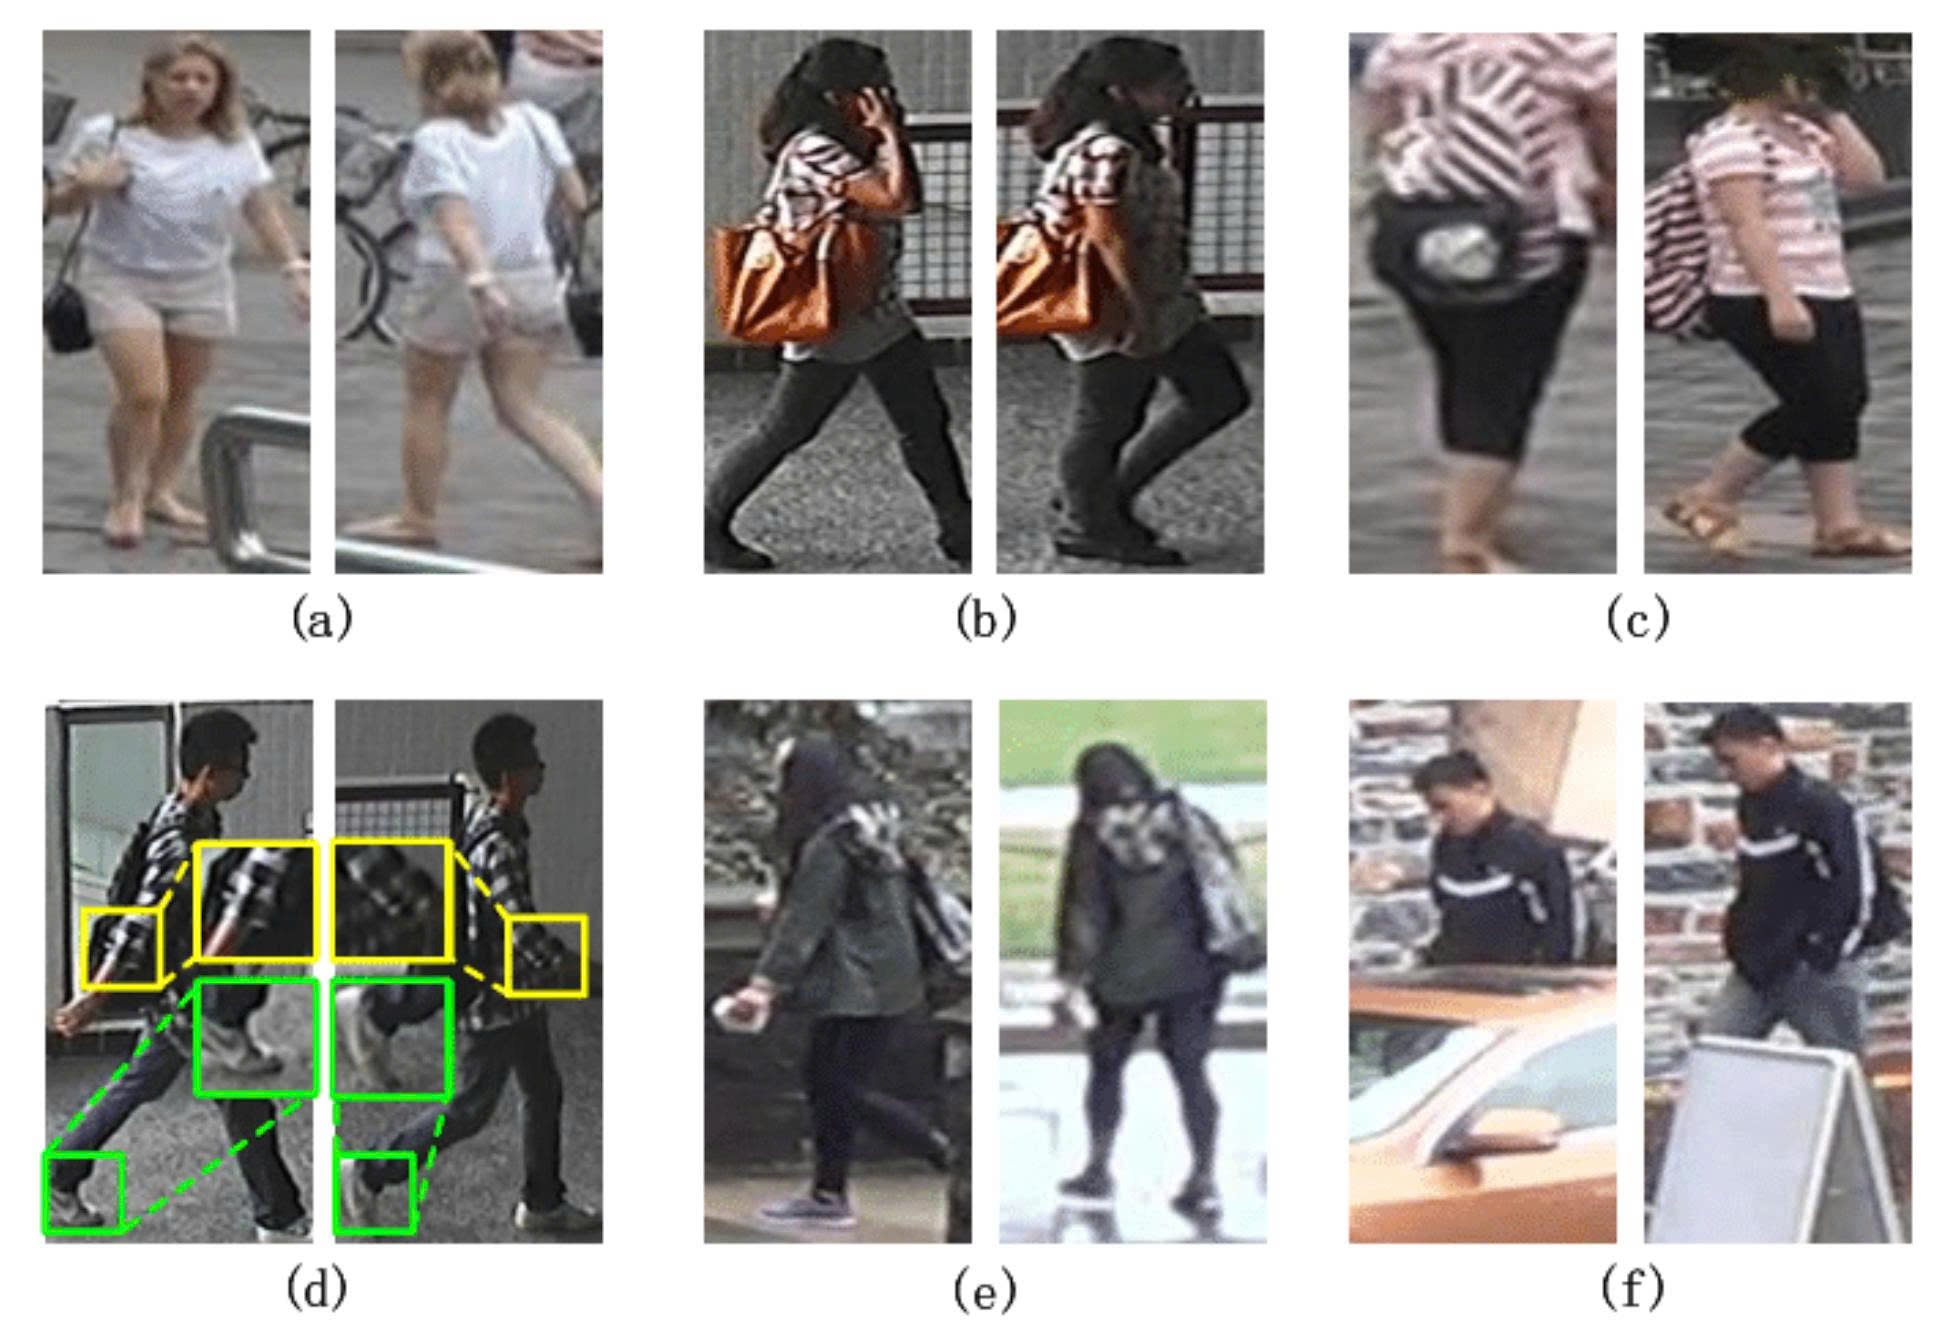
\includegraphics[width=0.5\textwidth]{img/person-re-identification-challenges.jpg}
    \caption{Một số thách thức chính trong bài toán Person Re-identification, bao gồm thay đổi góc nhìn, tư thế, che khuất và nền nhiễu.}
    \label{fig:reid_challenges}
\end{figure}

Từ đó, đề tài đặt ra các vấn đề chính cần xem xét: các hướng tiếp cận hiện có giải quyết bài toán này như thế nào, mô hình nào phù hợp để áp dụng trong phạm vi đồ án, và những cải tiến nào có thể giúp nâng cao hiệu quả nhận dạng khi thực nghiệm trên tập dữ liệu chuẩn.
